\documentclass[sigconf, nonacm]{acmart}

\AtBeginDocument{%
  \providecommand\BibTeX{{Bib\TeX}}}

\setcopyright{none}
\acmConference[Course Project]{Course Project Report}{}{}

\usepackage{tikz}
\usetikzlibrary{arrows.meta, positioning}
\emergencystretch=3em

\begin{document}

\title{Retrieval Strategy, Not Just Retrieval: A Controlled Comparison of RAG Pipelines for Detecting Malicious PyPI Packages}

\author{First Author}
\authornote{These authors contributed equally to this research.}
\email{first.author@institution.edu}
\orcid{0000-0000-0000-0000}
\affiliation{%
  \institution{Institution Name}
  \city{City}
  \state{State}
  \country{Country}
}

\author{Second Author}
\authornotemark[1]
\email{second.author@institution.edu}
\orcid{0000-0000-0000-0000}
\affiliation{%
  \institution{Institution Name}
  \city{City}
  \state{State}
  \country{Country}
}

\author{Third Author}
\authornotemark[1]
\email{third.author@institution.edu}
\orcid{0000-0000-0000-0000}
\affiliation{%
  \institution{Institution Name}
  \city{City}
  \state{State}
  \country{Country}
}

\author{Fourth Author}
\authornotemark[1]
\email{fourth.author@institution.edu}
\orcid{0000-0000-0000-0000}
\affiliation{%
  \institution{Institution Name}
  \city{City}
  \state{State}
  \country{Country}
}

\author{Fifth Author}
\correspondingauthor
\authornotemark[1]
\email{fifth.author@institution.edu}
\orcid{0000-0000-0000-0000}
\affiliation{%
  \institution{Institution Name}
  \city{City}
  \state{State}
  \country{Country}
}

\renewcommand{\shortauthors}{First Author et al.}

\begin{abstract}
Large language models (LLMs) can inspect source code for malicious behavior,
but they miss subtle attacks such as obfuscated droppers and typosquats whose
installation scripts look innocuous. Retrieval-augmented generation (RAG)
has been proposed as the remedy, yet prior work couples retrieval to
particular knowledge sources and mechanisms, leaving it unclear how much of
the benefit comes from retrieval itself and how much from how retrieval is
done. We isolate retrieval strategy through a controlled comparison of seven
pipelines---a zero-shot baseline and six RAG variants (dense, sparse BM25,
hybrid fusion, behavior-summary, contrastive dual-pool, and their
combination)---using the same LLM backbone, prompting, and code-only
knowledge base throughout, and evaluate on 1{,}020 test packages. We find
that code-level retrieval substantially improves detection, driven by a
large recall gain; simple sparse retrieval performs on par with heavy dense retrieval;
contrastive retrieval sharply reduces false alarms; and behavior-summary
queries are actively harmful. We also analyze the samples that no method
detects (metadata-cloned typosquats) and use a static-grounding proxy to
measure explanation faithfulness, showing that retrieval reduces unsupported
behavior claims.
\end{abstract}
\endinput


\begin{CCSXML}
<ccs2012>
 <concept>
  <concept_id>10011007.10011074.10011075</concept_id>
  <concept_desc>Software and its engineering~Software development techniques</concept_desc>
  <concept_significance>500</concept_significance>
 </concept>
 <concept>
  <concept_id>10002978.10003029.10011703</concept_id>
  <concept_desc>Security and privacy~Systems security~Vulnerability management</concept_desc>
  <concept_significance>300</concept_significance>
 </concept>
</ccs2012>
\end{CCSXML}

\ccsdesc[500]{Software and its engineering~Software development techniques}
\ccsdesc[300]{Security and privacy~Systems security~Vulnerability management}
\keywords{supply chain, malicious package, PyPI, large language model, RAG, retrieval, typosquatting}

\maketitle

\section{Introduction}
\label{sec:introduction}

Open-source package registries such as PyPI are a primary vector for software
supply-chain attacks: adversaries publish packages that masquerade as popular
libraries---through typosquatting, name squatting, or dependency
confusion---and execute malicious code during installation.
Studies of real-world registries have documented thousands of such
incidents~\cite{duan2021supply, ohm2020backstabber}, and the attack surface
keeps growing because anyone can publish, and installation scripts
(\texttt{setup.py}) are arbitrary code. Manual review does not scale, which
has motivated static-analysis heuristics and, more recently, large language
models (LLMs) that classify source code as malicious or benign.

LLMs are promising but imperfect reviewers: an 8B-scale instruct model is
strong at recognizing overt malware, yet it misses subtle cases such as
obfuscated droppers or typosquats whose installation script looks, on its
face, like any other package~\cite{ease2025rag}. One prominent remedy is
retrieval-augmented generation (RAG): before deciding, show the model
similar examples retrieved from a corpus of previously seen
malware~\cite{ease2025rag, crag2024}. Recent work applying RAG to malicious
PyPI package detection, most directly the EASE 2025 study ``Detecting
Malicious Source Code in PyPI Packages with LLMs: Does RAG Come in
Handy?''~\cite{ease2025rag}, reports that retrieved context improves detection,
but that study coupled retrieval to particular knowledge sources (external
threat-intelligence collections such as YARA rules and GitHub advisories) and
a single retrieval mechanism, leaving an important question open: \emph{how
much of the benefit comes from retrieval itself, and how much from how
retrieval is done?}

\begin{figure}[!ht]
    \centering
    \fbox{%
    \begin{minipage}[c]{0.995\linewidth}
        \centering
        \emph{Research question.}
        Given a fixed code-only knowledge base and a fixed LLM,
        which retrieval strategy---none, dense, sparse, hybrid,
        behavior-based, or contrastive---best detects malicious PyPI packages,
        and how do the strategies trade off recall, false alarms,
        and explanation faithfulness?
    \end{minipage}%
    }
    \caption{The research question addressed in this paper.}
    \label{fig:rq}
    \Description{Boxed statement of the paper's research question comparing
    retrieval strategies for malicious package detection.}
\end{figure}

This paper reports a controlled comparison of seven pipelines that differ
only in their retrieval strategy, evaluated on the same dataset used by the
EASE 2025 study, with a single fixed LLM (\texttt{Llama-3.1-8B-Instruct})
and a knowledge base built purely from the dataset's own training partition.
Our results show that:

\begin{itemize}
    \item \textbf{Any code-level retrieval is a large win.} Dense or sparse
    retrieval lifts malicious-class F1 from 0.888 (no RAG) to 0.968--0.972
    (+8 points), driven almost entirely by a 17-point recall gain
    (0.798~$\rightarrow$~0.972).
    \item \textbf{Sparse retrieval suffices.} Plain BM25 over source tokens
    matches a 4B embedding model within 0.4 F1 points, and hybrid fusion of
    the two does not improve on the better single retriever.
    \item \textbf{Contrastive retrieval minimizes false alarms.} Retrieving
    benign counterexamples alongside malicious ones lowers the false-positive
    rate from 0.8--1.2\% to 0.1\% while preserving 0.948 recall and
    0.996 precision.
    \item \textbf{AST behavior summaries are lossy.} Representing code as
    extracted behavior summaries for retrieval \emph{hurts}
    (F1 0.878), below even the no-RAG baseline.
\end{itemize}

\section{Motivation}
\label{sec:motivation}

Two practical concerns motivate the comparison. First, deployment cost:
if a lexicon index suffices, teams can skip embedding infrastructure,
vector stores, and the associated hosting budget. Second, triage cost:
security-reviewing LLM-predicted alarms is expensive, so the false-positive
rate per millisecond-of-recall may matter more than raw F1. By measuring
recall, false alarms, coverage (parse failures), and explanation grounding
side by side, we aim to give practitioners---and follow-up researchers---a
basis to choose a retrieval strategy on purpose rather than by habit.

\section{Contributions}
\label{sec:contributions}

The main contributions of this paper are:
\begin{itemize}
    \item A controlled, reproducible comparison of six RAG variants plus a
    zero-shot baseline (E0--E6) for LLM-based detection of malicious PyPI
    packages on the EASE 2025 dataset, isolating retrieval strategy as the
    only varying factor.
    \item Evidence that sparse retrieval matches dense retrieval on this
    task (0.968 vs.\ 0.972 F1) with no learned components.
    \item Evidence that contrastive dual-pool retrieval reduces false alarms
    by an order of magnitude at modest recall cost.
    \item A negative result for behavior-summary retrieval, quantifying what
    is lost when code is reduced to AST-derived descriptions.
    \item An analysis of replication-grade failure modes: samples no method
    detects (metadata-cloned typosquats), recurring false positives, and
    structured-output parse failures, with per-sample raw outputs and a
    reproducible evaluation pipeline released as a replication package.
\end{itemize}

\section{Paper Structure}
\label{sec:structure}

The remainder of this paper is structured as follows.
Section~\ref{sec:related-work} reviews related work on supply-chain attacks,
LLMs for malicious-code detection, and retrieval-augmented methods.
Section~\ref{sec:methodology} details the dataset, the seven retrieval
strategies, the LLM configuration, and the evaluation metrics.
Section~\ref{sec:results} presents the main results, fairness-oriented
faithfulness statistics, and an error analysis. Section~\ref{sec:discussion}
interprets the findings, discusses limitations and threats to validity, and
outlines future work. Section~\ref{sec:conclusion} concludes.
\endinput

\section{Related Work}
\label{sec:related-work}

\subsection{Supply-Chain Attacks on Package Registries}
\label{sec:supply-chain}

Malicious publications in package registries are a well-documented,
persistent threat. Duan et al.~\cite{duan2021supply} measured hundreds of
malicious packages across PyPI, npm, and RubyGems, showing that most are
installed by ordinary users through ordinary \texttt{pip install}-style
commands, and that name-based imitation (typosquatting) is a dominant attack
style. Ohm et al.~\cite{ohm2020backstabber} cataloged attack techniques in
open-source software supply chains, including injections that trigger at
package-install time through \texttt{setup.py} hooks. Empirical studies of
the PyPI ecosystem report that malicious packages persist despite
registry-level safeguards~\cite{guo2023pypi, liang2021malicious}, and
graph-based and behavior-modeling approaches have been proposed for
detecting them in adjacent ecosystems~\cite{huang2024spiderscan}. Industry
efforts such as Datadog's malicious-software-packages
dataset~\cite{datadog-dataset} have made labeled collections of such
packages publicly available, which we use here.

\subsection{LLMs for Malicious-Code Detection}
\label{sec:llm-detection}

Recent work applies LLMs to security classification tasks. Studies on
vulnerability reasoning caution that LLMs remain unreliable on subtle
security judgments without auxiliary signal~\cite{ullah2024llmsec}. For
malicious packages specifically, LLMs have been used to detect malware in
the npm ecosystem~\cite{zahan2024npm}, and Ibiyo et al.~\cite{ease2025rag}---the closest
prior work to ours---evaluated LLMs with zero-shot prompting, RAG, and
few-shot learning on a dataset of malicious and benign PyPI
packages~\cite{ease2025rag}. Its knowledge bases were built from YARA rules,
GitHub security advisories, and malicious \texttt{setup.py} examples. A
central finding of that study was counterintuitive: retrieval augmentation
did not reliably help, yielding mediocre accuracy, whereas few-shot learning
was markedly more effective. The study, however, coupled retrieval to its
specific knowledge sources and a single retrieval mechanism, so it does not
separate the effect of \emph{whether} to retrieve from \emph{how} retrieval
is done.
A complementary line of work applies multi-agent LLM pipelines to
package-level evidence such as metadata and behavioral descriptions,
reporting improvements from aggregating multiple signals (\texttt{LAMPS},
``Many Hands Make Light Work'')~\cite{lamps2026}. Our work differs in scope
and design: instead of changing the knowledge source or inventing new
pipelines, we fix the corpus, the model, and the prompt, and vary only the
retrieval strategy, which lets us attribute performance differences to
retrieval design rather than to data or agent orchestration.

\subsection{Retrieval and Retrieval-Augmented Generation}
\label{sec:rag}

Retrieval-augmented generation combines a retriever with a generator so that
the model conditions on relevant external evidence~\cite{lewis2020rag,
gao2023ragsurvey}. Dense passage retrieval established embedding-based
retrieval as a standard for open-domain question answering~\cite{dpr2020};
in parallel, classical sparse scoring, notably the Okapi BM25 function,
remains a strong lexical baseline with a well-understood probabilistic
foundation~\cite{bm252009}. Hybrid systems fuse the two, most simply with
Reciprocal Rank Fusion~\cite{rrf2009}. Within security, RAG has been applied
to vulnerability detection in smart contracts~\cite{yu2024smartcontract} and
to knowledge-level augmentation of LLM vulnerability analysis with
CVE-derived documents~\cite{du2024vulrag}. For malicious code specifically,
retrieving code examples has been the first thing
tried~\cite{ease2025rag, crag2024}, yet---to our knowledge---no prior study
has systematically compared dense, sparse, hybrid, behavior-based, and
contrastive retrieval configurations on the same malicious-package benchmark
with the same generator. This is the gap we address.

\subsection{Summary}
\label{sec:related-summary}

In summary, prior work (i)~established the supply-chain threat and the
datasets we build on, (ii)~showed that LLMs augmented with retrieved
knowledge are promising but not sufficient for malicious-package detection,
and (iii)~provides the retrieval toolbox (dense, sparse, fusion). Our
contribution is a controlled, seven-condition comparison that isolates
retrieval strategy, together with faithfulness-oriented evaluation of the
model's behavior claims, on the same data and model family used by
Ibiyo et al.~\cite{ease2025rag}.
\endinput

\section{Methodology}
\label{sec:methodology}

\subsection{Overview}
\label{sec:method-overview}

We study whether, and how, retrieval-augmented generation (RAG) improves an
LLM's ability to detect malicious PyPI packages, by comparing seven
alternative pipelines~E0--E6 that differ only in the \emph{retrieval strategy}
they apply before the final classification. At a high level, every pipeline
(1)~takes the target package's \texttt{setup.py} source as input,
(2)~builds a query representation from it,
(3)~optionally retrieves reference examples from a knowledge base of
previously seen packages,
(4)~feeds the target together with the retrieved evidence (if any) to an
instruction-tuned LLM, and
(5)~asks the model for a structured verdict: malicious or benign, a confidence
score, security-relevant behaviors with source-line citations, and a rationale.
Figure~\ref{fig:pipeline} illustrates the pipeline.

\begin{figure}[!ht]
    \centering
    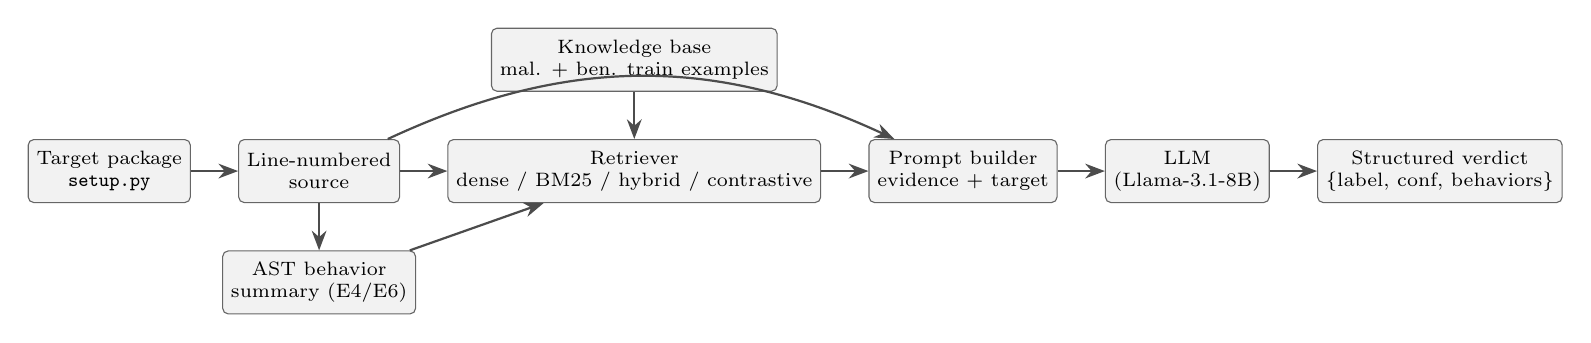
\begin{tikzpicture}[
        node distance=6mm,
        box/.style={rectangle, rounded corners=2pt, draw=black!60, fill=gray!10,
                    minimum height=8mm, align=center, font=\scriptsize,
                    inner sep=3pt},
        arr/.style={-{Stealth[length=2.5mm]}, thick, black!70},
    ]
    \node[box] (target) {Target package \\ \texttt{setup.py}};
    \node[box, right=of target] (num) {Line-numbered \\ source};
    \node[box, below=of num] (beh) {AST behavior \\ summary (E4/E6)};
    \node[box, right=of num] (ret) {Retriever \\ dense / BM25 / hybrid / contrastive};
    \node[box, above=of ret] (kb) {Knowledge base \\ mal. + ben. train examples};
    \node[box, right=of ret] (prompt) {Prompt builder \\ evidence + target};
    \node[box, right=of prompt] (llm) {LLM \\ (Llama-3.1-8B)};
    \node[box, right=of llm] (out) {Structured verdict \\ \{label, conf, behaviors\}};
    \draw[arr] (target) -- (num);
    \draw[arr] (num) -- (ret);
    \draw[arr] (num) -- (beh);
    \draw[arr] (beh) -- (ret);
    \draw[arr] (kb) -- (ret);
    \draw[arr] (ret) -- (prompt);
    \draw[arr] (num) to[out=25, in=155] (prompt);
    \draw[arr] (prompt) -- (llm);
    \draw[arr] (llm) -- (out);
    \end{tikzpicture}
    \caption{Overview of the evaluated pipelines. All stages are shared across
    methods except query construction and retrieval (E4/E6 additionally build an
    AST behavior summary as the query).}
    \label{fig:pipeline}
    \Description{Pipeline with target package input, line numbering,
    optional AST behavior summary, retrieval from a knowledge base, prompt
    construction, an LLM call, and a structured verdict output.}
\end{figure}

\subsection{Dataset}
\label{sec:dataset}

We reuse the dataset assembled in the EASE~2025 study on RAG for malicious
code detection~\cite{ease2025rag}, which itself mines packages from Datadog's
malicious-software-packages dataset~\cite{datadog-dataset}. The replication
package ships pre-split JSON files: a training partition of 1{,}158 malicious
and 3{,}005 benign packages, and a test partition of 276 malicious and 753
benign packages (1{,}029 in total). Each entry contains
the package name, file list, and the raw \texttt{setup.py} content; test
entries additionally carry an AST-derived textual behavior description.
Nine malicious test entries whose \texttt{setup.py} could not be extracted
(content string \texttt{"Not Available"}) are excluded from evaluation,
leaving 1{,}020 test samples. The training partition serves as the knowledge
base; the test partition is never used for retrieval.

The malicious class is dominated by typosquatted or squatted packages
(e.g.,~\texttt{colorama} clones, \texttt{requests}-lookalikes) whose
installation code frequently hides its malicious behavior in the
\texttt{setup.py} entry point. This makes the task representative of
real-world supply-chain attacks that LLM-based tooling is expected to catch.

\subsection{Retrieval Strategies}
\label{sec:retrieval}

All methods share the same knowledge base: the raw \texttt{setup.py} sources
of the 4{,}163 training packages, indexed in separate malicious and benign
pools. We fix the number of retrieved documents to $k=3$, following the
reference design. The seven methods are:

\begin{itemize}
    \item \textbf{E0 --- No RAG.} The target source is classified directly,
    without any retrieved context. This is the controlled baseline.
    \item \textbf{E1 --- Dense RAG.} The query is embedded with a sentence
    embedding model and matched by cosine similarity against the embedded
    training documents. We use the \texttt{Qwen3-Embedding-4B} model~\cite{qwen3emb}
    and a FAISS \texttt{IndexFlatIP} store over L2-normalized vectors~\cite{vllm2023}.
    \item \textbf{E2 --- BM25 RAG.} Sparse lexical retrieval with the
    Okapi BM25 scoring function~\cite{bm252009}; no learned components.
    \item \textbf{E3 --- Hybrid RAG.} Dense (E1) and sparse (E2) rankings are
    fused with Reciprocal Rank Fusion~\cite{rrf2009},
    $\sum_r 1/(60 + \mathrm{rank}_r(d))$; no fusion weights are trained.
    \item \textbf{E4 --- Behavior RAG.} The target is represented by a static
    behavior summary---imports, suspicious API calls, and behaviors such as
    shell execution, network access, dynamic execution, or base64 decoding,
    extracted with Python's \texttt{ast} module---and dense retrieval runs over
    behavior summaries of the malicious pool, analogous to the
    AST descriptions used in the original dataset.
    \item \textbf{E5 --- Contrastive RAG.} Dense retrieval is run twice:
    top-$k$ documents from the malicious pool \emph{and} top-$k$ from the
    benign pool, and both groups are shown to the model with explicit
    \texttt{MAL}/\texttt{BEN} markers.
    \item \textbf{E6 --- Behavior + Contrastive RAG.} Behavior-summary
    queries (as in E4) combined with dual-pool contrastive evidence (as in E5).
\end{itemize}

\subsection{LLM Configuration and Prompting}
\label{sec:llm-config}

Classification is performed by \texttt{Llama-3.1-8B-Instruct}~\cite{llama3}
served through an OpenAI-compatible vLLM endpoint~\cite{vllm2023}. Generation
uses temperature $0$ and a maximum of 1{,}024 output tokens. The system prompt
instructs the model that it is performing static source-code analysis, not to
assume behavior unsupported by the source or retrieved evidence, and that
retrieved examples are references rather than proof; every claimed behavior
must cite target source lines. The target source is line-numbered before it is
embedded in the prompt. The output schema is enforced as JSON and requires
\texttt{verdict} (malicious/benign), \texttt{confidence},
\texttt{behaviors} (a list of \{type, evidence\} objects) and
\texttt{rationale}. Retrieved documents are labeled with stable identifiers
(\texttt{MAL\_*} / \texttt{BEN\_*}) and their retrieval scores.

\subsection{Evaluation Metrics}
\label{sec:metrics}

\paragraph{Classification.} We report precision, recall, and F1 for the
malicious class, benign-class F1, macro-F1, balanced accuracy, false-positive
rate (FPR), and false-negative rate (FNR). Because JSON decoding can fail
(e.g., output truncation by the serving backend), we additionally report
\emph{coverage}: the fraction of samples whose response parsed successfully;
unparsed samples are counted as failures and excluded from metric
denominators, so that success and failure modes are reported separately.

\paragraph{Explanation faithfulness.} As an approximation of whether the
model ``hallucinates'' security-relevant behaviors, we ground each claimed
behavior in a lightweight static checker built on Python's \texttt{ast}
module, which flags shell execution, process creation, network access, file
writes/deletion, dynamic execution, environment access, base64 decoding,
remote download, and persistence. Free-form behavior names produced by the
model are keyword-normalized to this vocabulary; a claim is
\emph{supported} when the corresponding static flag is present on any line of
the target. We report the unsupported-claim rate
$= \mathrm{unsupported} / \mathrm{claimed}$, behavior precision and behavior
recall. Because static analysis is neither sound nor complete on obfuscated
code, we treat these figures as an \emph{automated static-grounding proxy},
not as hallucination ground truth.

\subsection{Implementation and Reproducibility}
\label{sec:implementation}

The pipeline is implemented in Python 3.12 as a modular package
(retrieval, static analysis, prompting, evaluation modules) without
framework dependencies; BM25 uses \texttt{rank-bm25}, dense indexes use
\texttt{faiss}, and LLM/embedding calls go through a single
OpenAI-compatible client so that any endpoint can be swapped by environment
variables. All LLM responses, embeddings, and retrieval results are cached
(SQLite) keyed by prompt hash, sample content, evidence IDs, and generation
parameters; retrieval indexes are persisted on disk; and every run records
its configuration, seed, model IDs, and git commit. Run scripts for all seven
methods, the evaluation code, and raw per-sample outputs are included in the
replication package.
\endinput

\section{Results}
\label{sec:results}

\subsection{Experimental Setup}
\label{sec:experimental-setup}

Description of datasets, baselines, metrics, and hardware.

\subsection{Main Results}
\label{sec:main-results}

Presentation of main experimental results.

\begin{table}[htbp]
    \caption{Main results comparison.}
    \label{tab:main-results}
    \begin{tabular}{lccc}
        \toprule
        \textbf{Method} & \textbf{Metric 1} & \textbf{Metric 2} & \textbf{Metric 3} \\
        \midrule
        Baseline 1 & 0.85 & 0.72 & 0.91 \\
        Baseline 2 & 0.88 & 0.75 & 0.93 \\
        \textbf{Ours} & \textbf{0.92} & \textbf{0.81} & \textbf{0.96} \\
        \bottomrule
    \end{tabular}
\end{table}

\subsection{Ablation Study}
\label{sec:ablation}

Ablation study results.

\subsection{Qualitative Analysis}
\label{sec:qualitative}

Qualitative examples and analysis.
\endinput
\section{Discussion}
\label{sec:discussion}

\subsection{Interpretation of Results}
\label{sec:interpretation}

Discussion of what the results mean.

\subsection{Limitations}
\label{sec:limitations}

Limitations of your work:
\begin{itemize}
    \item Limitation 1
    \item Limitation 2
    \item Limitation 3
\end{itemize}

\subsection{Threats to Validity}
\label{sec:threats}

Threats to internal, external, and construct validity.

\subsection{Future Work}
\label{sec:future-work}

Directions for future research.
\endinput
\section{Conclusion}
\label{sec:conclusion}

This paper asked what retrieval strategy, if any, best supports LLM-based
detection of malicious PyPI packages. Using the EASE 2025 dataset, a fixed
\texttt{Llama-3.1-8B-Instruct} generator, and a code-only knowledge base, we
compared a zero-shot baseline against dense, sparse, hybrid, behavior-based,
and contrastive retrieval.

Three conclusions appear robust. Any code-level retrieval is a large win,
lifting malicious-class F1 from 0.888 to 0.97, mostly through recall. The
mechanism matters surprisingly little: plain BM25 matches a 4B embedding
retriever within 0.4 F1 points, so sparse retrieval is a strong, low-cost
default. And contrastive retrieval offers a favorable precision/recall
trade-off: retrieving benign counterexamples cuts the false-positive rate to
0.1\% at 0.948 recall. Conversely, reducing queries to AST behavior summaries
is counterproductive (F1 0.878), demonstrating that signal loss in query
construction, not retrieval per se, is where methods fail.

We also documented the residual failures that no retrieval over
\texttt{setup.py} can fix---metadata-cloned typosquats---and the recurring
false positives over security-adjacent legitimate packages, as guidance for
the next generation of designs, which should extend evidence beyond a single
file, add name-level signals, and calibrate retrieval toward triage
workflows.
\endinput


\begin{acks}
Acknowledgments here.
\end{acks}

\bibliographystyle{ACM-Reference-Format}
\bibliography{references}

\end{document}
\endinput